\section{Scalability}\label{section:scalability}

In order to evaluate the scalability of our application, we prepared a production environment that is appropriate for handling the number of concurrent users to be expected in a \mooc. We simulated a corresponding load using Apache JMeter\foo{http://jmeter.apache.org/}.

\subsection{Test Environment}

The production server is equipped with two Intel Xeon E5-2680 v2\foo{http://ark.intel.com/products/75277} \glspl{cpu}, supplying 40 logical \gls{cpu} cores in total, and 64 GB of memory.

The server hosts all major components of \tool, which are the web application, a web server, the database, and Docker. We use Ubuntu 14.04.1 LTS (64-bit), Docker 1.3.1, and PostgreSQL 9.3.5. As depicted in Figure~\ref{figure:server}, the web application is served by Puma\foo{http://puma.io/} 2.10.1, a web server built for speed and concurrency, using Nginx\foo{http://nginx.org/} 1.6.2 as a reverse proxy.

\begin{figure}
\centering
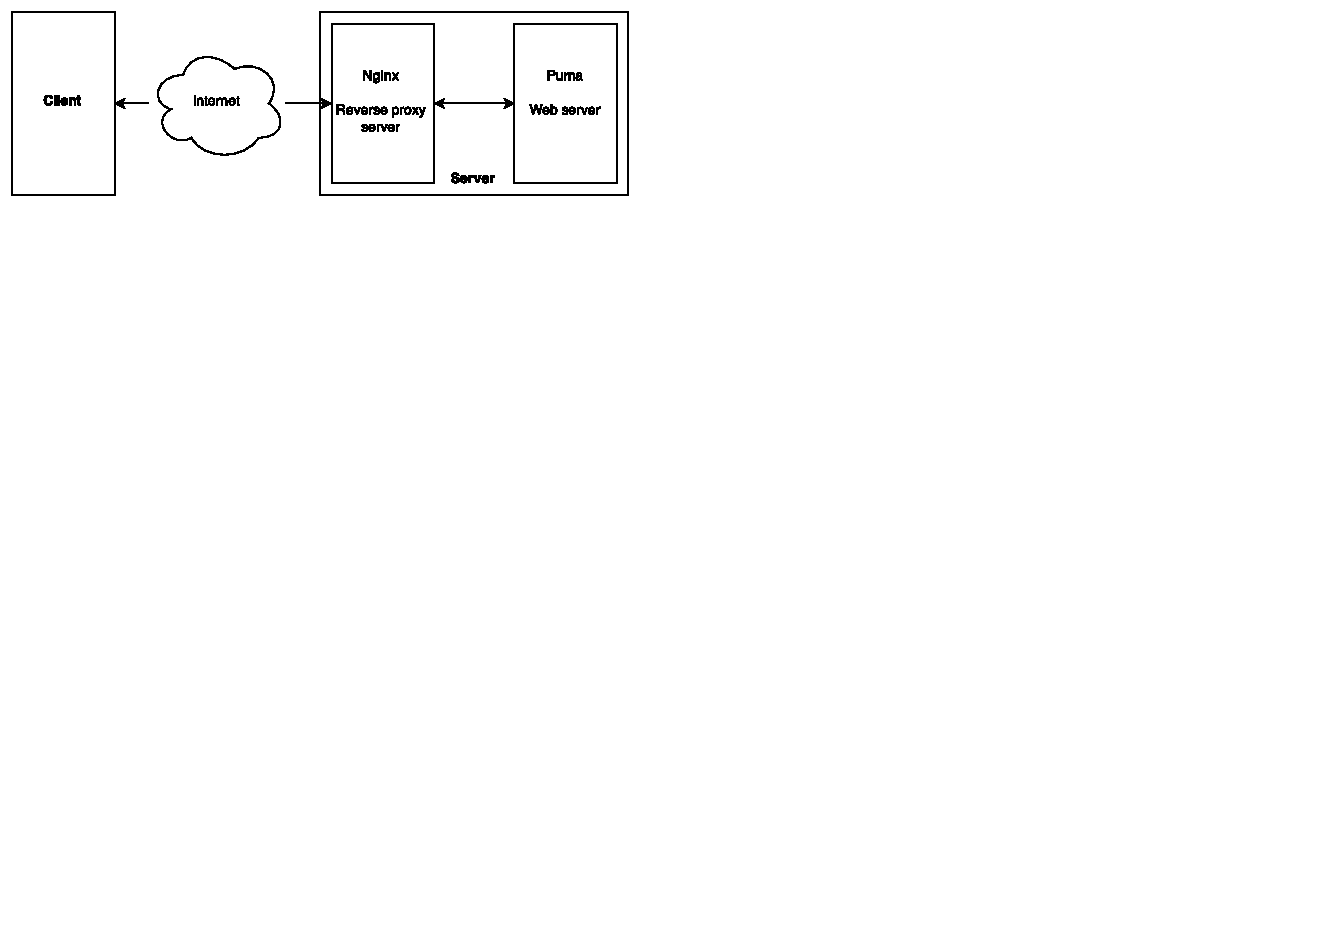
\includegraphics[clip=true, trim=0.1cm 12.7cm 11.8cm 0.1cm, width=\textwidth]{images/server.pdf}
\caption{Web Server Setup}
\label{figure:server}
\end{figure}

In order to make best use of the parallelism provided by the server's many-core \gls{cpu}, we decided not to use Ruby's standard interpreter, which is \gls{mri}, but to rely on JRuby, its \gls{jvm}-based equivalent. While \gls{mri}'s \gls{gil} limits the multi-thread performance of a single interpreter process by allowing only one thread to execute at a time~\cite{odaira2014eliminating}, JRuby offers thread-level parallelism by mapping Ruby threads to Java threads, which in turn are mapped to native \gls{os} threads by most \glspl{jvm}.

In order to prepare the production environment for the planned load, we set the maximum numbers of database connections allowed by PostgreSQL and allocatable by Active Record's connection pool\foo{http://api.rubyonrails.org/classes/ActiveRecord/ConnectionAdapters/ConnectionPool.html} to 1024. Moreover, Puma has been configured to use up to 64 threads.

\subsection{Test Plan}

The JMeter-based load test simulates 500 learners who use \tool in parallel to solve a practical assignment.

Each simulated student's programming session starts with an \gls{lti} launch request, as described in Section~\ref{section:interoperability2}. After that, students perform an iterative development process, as discussed in Section~\ref{section:development-environment3}. Each iteration comprises two requests between client and server. The first request sends the learner's code to the server for creating a code snapshot. The second request triggers either a code run or the execution of tests.

The requests associated to a single simulated student are issued at intervals of five seconds, which mimic the student's thinking time.

\subsection{Test Results}

\begin{figure}[h]
\centering
\hspace{-0.5cm}
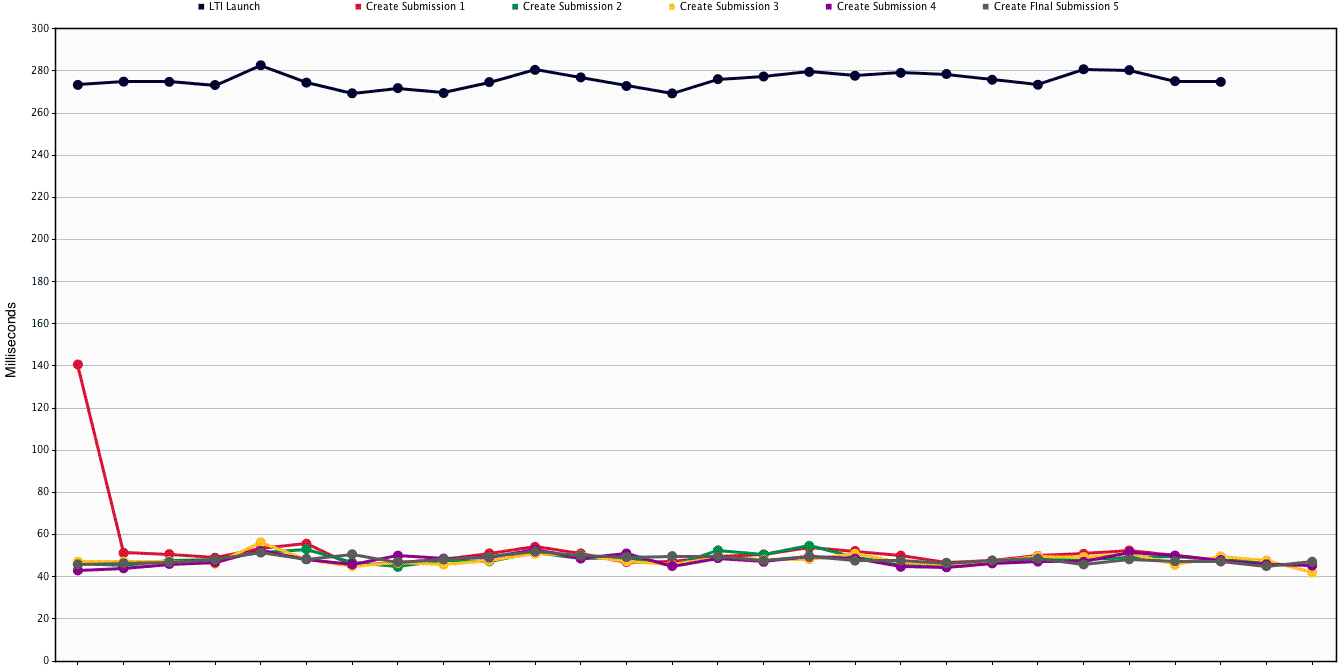
\includegraphics[width=0.9\textwidth]{images/jmeter1.png}
\caption{Response Time Graph Depicting Requests for \gls{lti} Launch and Snapshot Creation}
\label{figure:jmeter1}
\end{figure}

Figure~\ref{figure:jmeter1} depicts the response times of requests for starting the programming session and sending code revisions to the server. An \gls{lti} launch request, which involves validating the request signature, redirecting the learner to the specified exercise, and rendering the development environment, takes about 270 ms on average. The simpler request for creating a code submission, which does not render a view but yields a \gls{json} response, takes about 50 ms on average.

Short and hardly varying response times throughout the entire load test indicate that \tool is able to handle the simulated load for the regarded requests without problems. Moreover, the application should be able to handle a higher number of concurrent users when given a proportionate amount of resources.

\begin{figure}
\centering
\hspace{-0.5cm}
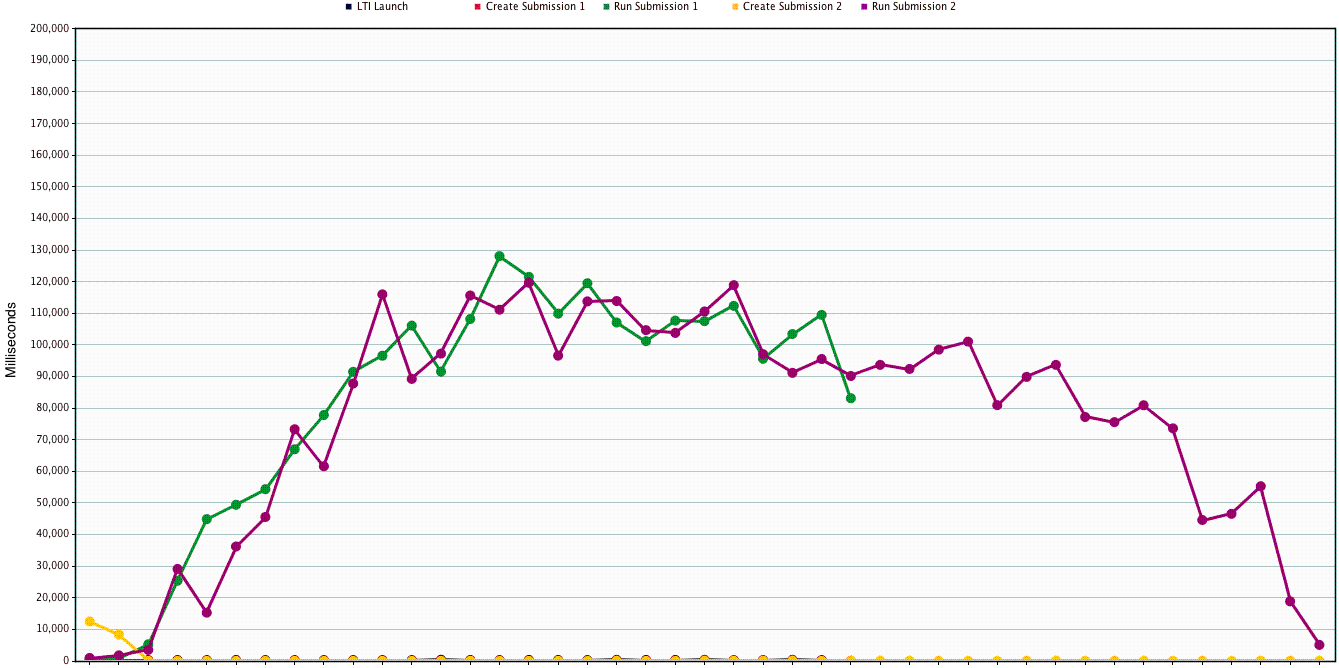
\includegraphics[width=0.9\textwidth]{images/jmeter2.png}
\caption{Response Time Graph Depicting Requests for \gls{lti} Launch, Snapshot Creation, and Code Execution}
\label{figure:jmeter2}
\end{figure}

Unfortunately, an entirely different picture emerges when taking code execution and assessment into account. Figure~\ref{figure:jmeter2} depicts the response times of a subset of the requests regarded in Figure~\ref{figure:jmeter1} as well as requests corresponding to code execution. As the graph in Figure~\ref{figure:jmeter2} shows, response times for code execution increase with the number of concurrent requests. In a massively parallel usage scenario, as simulated by the load test, response times rapidly reach a level at which students cannot be provided with feedback in a timely manner anymore. While concurrent requests increase the response times for code execution to tens of seconds, the response times of all other requests remain at similar levels as depicted in Figure~\ref{figure:jmeter1}. However, due to the increased range of response times, these requests are barely perceptible in Figure~\ref{figure:jmeter2}.

\begin{figure}
\centering
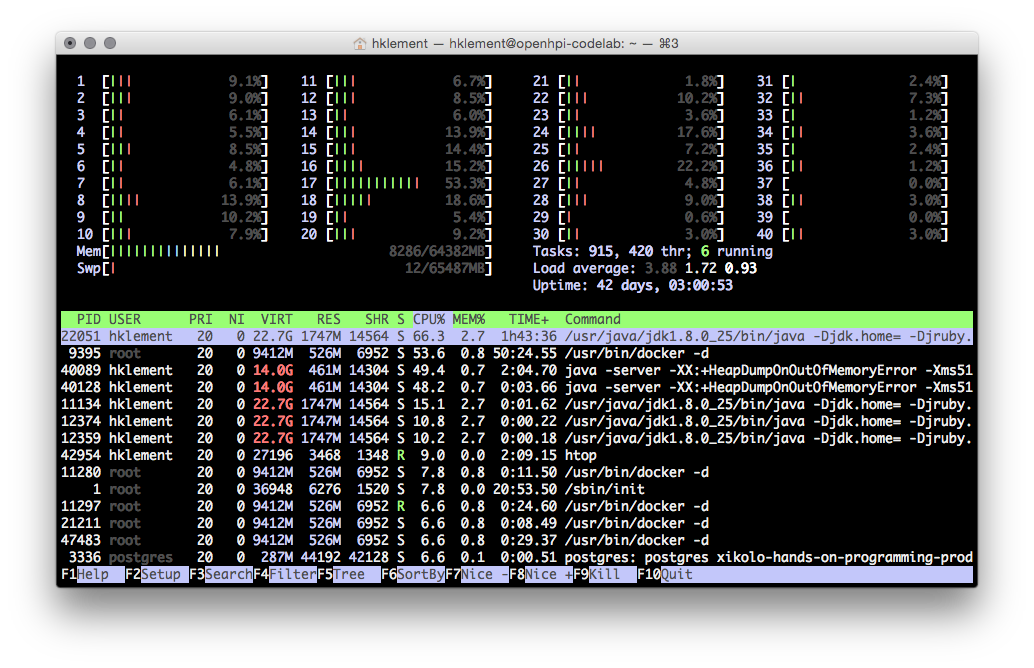
\includegraphics[width=0.9\textwidth]{images/htop1.png}
\vspace{-0.75cm}
\caption{Server Workload During the Load Test}
\label{figure:htop1}
\end{figure}

The fact that only Docker-related requests' response times escalate, while other requests are handled with ease, suggests that there is no general resource shortage but rather a problem concerning Docker. Figure~\ref{figure:htop1} shows the server's workload during the load test as determined using the process viewer htop\foo{http://hisham.hm/htop/}. In fact, the image does not indicate resource shortage, but it shows that the server's available \glspl{cpu} and memory are hardly used. Therefore, we believe that the poor scalability of code execution is attributable to problems with parallelizing server-to-server requests between the web application and Docker's \gls{api} endpoint.

\begin{figure}
\centering
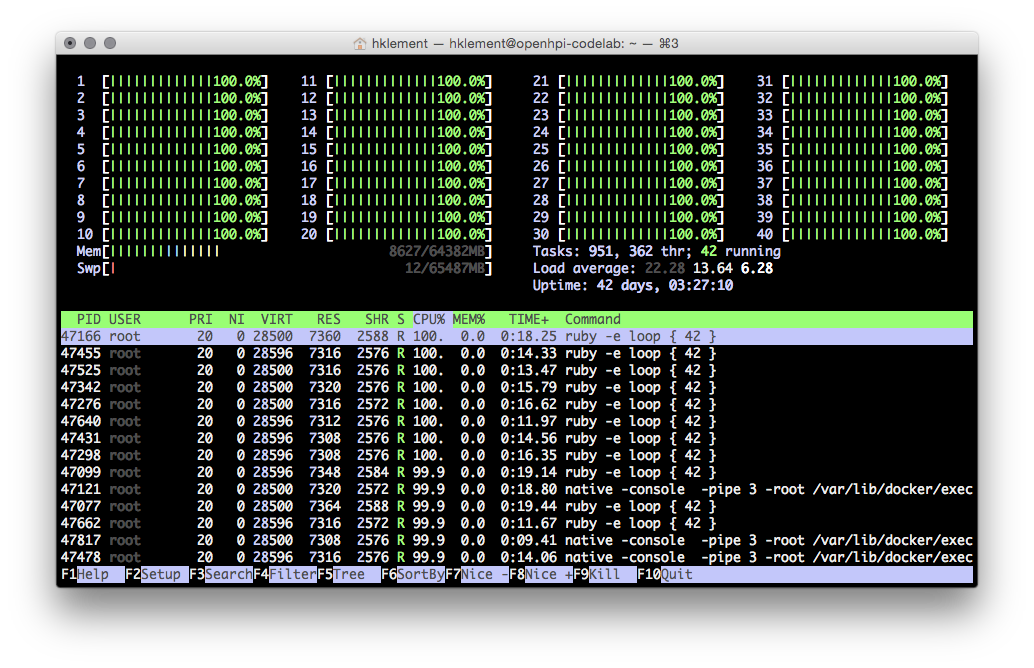
\includegraphics[width=0.9\textwidth]{images/htop2.png}
\vspace{-0.75cm}
\caption{Server Workload During the Parallelizability Experiment}
\label{figure:htop2}
\end{figure}

The production server's many-core \gls{cpu} should easily support running a sizable number of Docker containers in parallel. In order to eliminate the possibility of a general parallelization problem, we conducted an experiment investigating the parallelizability of concurrent Docker executions. In contrast to short-running processes, which are usual for students' code submissions and which are represented in the load test, we regarded the behavior of long-running processes executed in Docker containers. In order to minimize the differences between the load test and the experiment, containers were started from within \tool's web application. Figure~\ref{figure:htop2} depicts the server's workload during the experiment. The image shows that all logical \gls{cpu} cores are fully occupied by running the Docker containers. Hence, parallelization of concurrently running Docker containers is possible on the regarded infrastructure.

Based on our observations, we deduce that Docker can provide sandboxed execution of multiple learners' code submissions in parallel. While this should theoretically provide the scalability needed for a large-scale usage of \tool, scalable code execution is not achieved in practice. We suspect that the increasing response times for concurrent code execution requests are caused by a problem with parallelizing the allocation of new Docker containers. In order to enable the usage of \tool in a \mooc, this issue has yet to be eliminated or evaded.
